\documentclass[12pt]{beamer}

\usepackage[T2A]{fontenc}
\usepackage[utf8]{inputenc}
\usepackage[russian]{babel}
\usepackage{algorithm}
\usepackage{algpseudocode}
\usepackage{amssymb}
\usepackage{amsmath}
\usepackage{breqn}
\usepackage{enumerate}

\usepackage{graphicx}
\graphicspath{ {./} }

\def\multiset#1#2{\ensuremath{\left(\kern-.3em\left(\genfrac{}{}{0pt}{}{#1}{#2}\right)\kern-.3em\right)}}
\newcommand{\RNum}[1]{\uppercase\expandafter{\romannumeral #1\relax}}

\title{Моделирование внутриклеточного броуновского движения}
\author{Новиков Георгий}
\institute{Научный руководитель: \\Шпильман Алексей Александрович\\Академический университет}
\date{2016}

\begin{document}

\maketitle

\begin{frame}{Броуновское движение}
	Броуновское движение — беспорядочное движение взвешенных в жидкости или газе частиц. \\
	\begin{figure}
		\centering 
		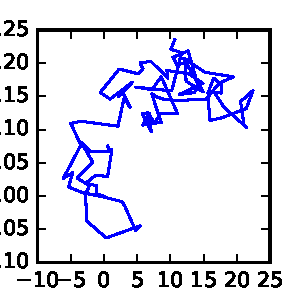
\includegraphics{br.pdf}
		\label{image2}
	\end{figure}
\end{frame}

\begin{frame}{Математическая модель}
	Для свободного броуновского движения:
	$$\Delta x \sim \mathcal{N}(0, \alpha \Delta t)$$
\end{frame}

\begin{frame}{Экспериментальные данные для клетки}
	Эксперимент показывает, что в клетке все не так:
	$$\Delta x \sim \mathcal{N}(0, \alpha (\Delta t)^\beta)$$
	\begin{figure}
		\centering 
		\scalebox{0.3}{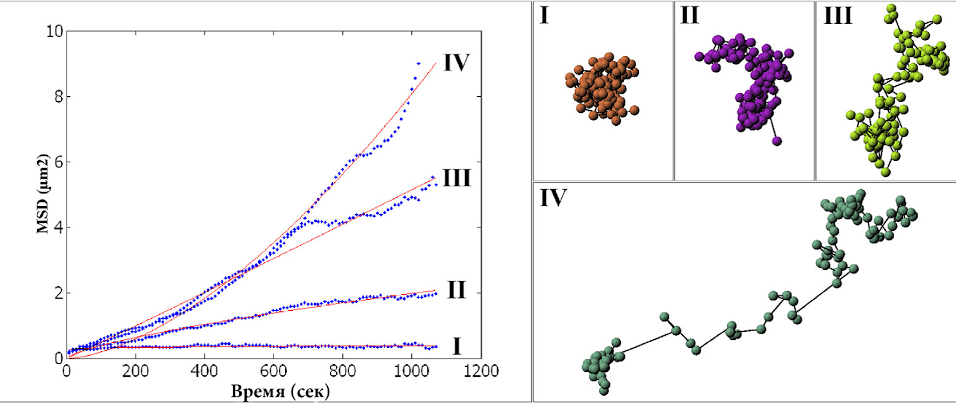
\includegraphics{brown.png}}
		\label{image2}
	\end{figure}
\end{frame}

\begin{frame}{Постановка задачи}
	Необходимо подобрать модель, наилучшим образом описывающую экспериментальные данные.
\end{frame}

\begin{frame}{Значение слова "описывать"}
	\begin{enumerate}
		\item Разделим экспериментальные частицы на $k$ групп (по размеру). 
		\item Внутри групп усредним значения $\alpha, \beta$ - получим вектор размера $2k$ - вектор признаков. 
		\item Для конкретной модели клетки при помощи моделирования можно посчитать ожидаемый вектор признаков. 
	\end{enumerate}
	Чем ближе ожидаемый вектор признаков к реальному - тем лучше модель объясняет экспериментальные данные.  
\end{frame}

\begin{frame}{Моделирование}
	\begin{figure}
		\centering 
		\scalebox{0.18}{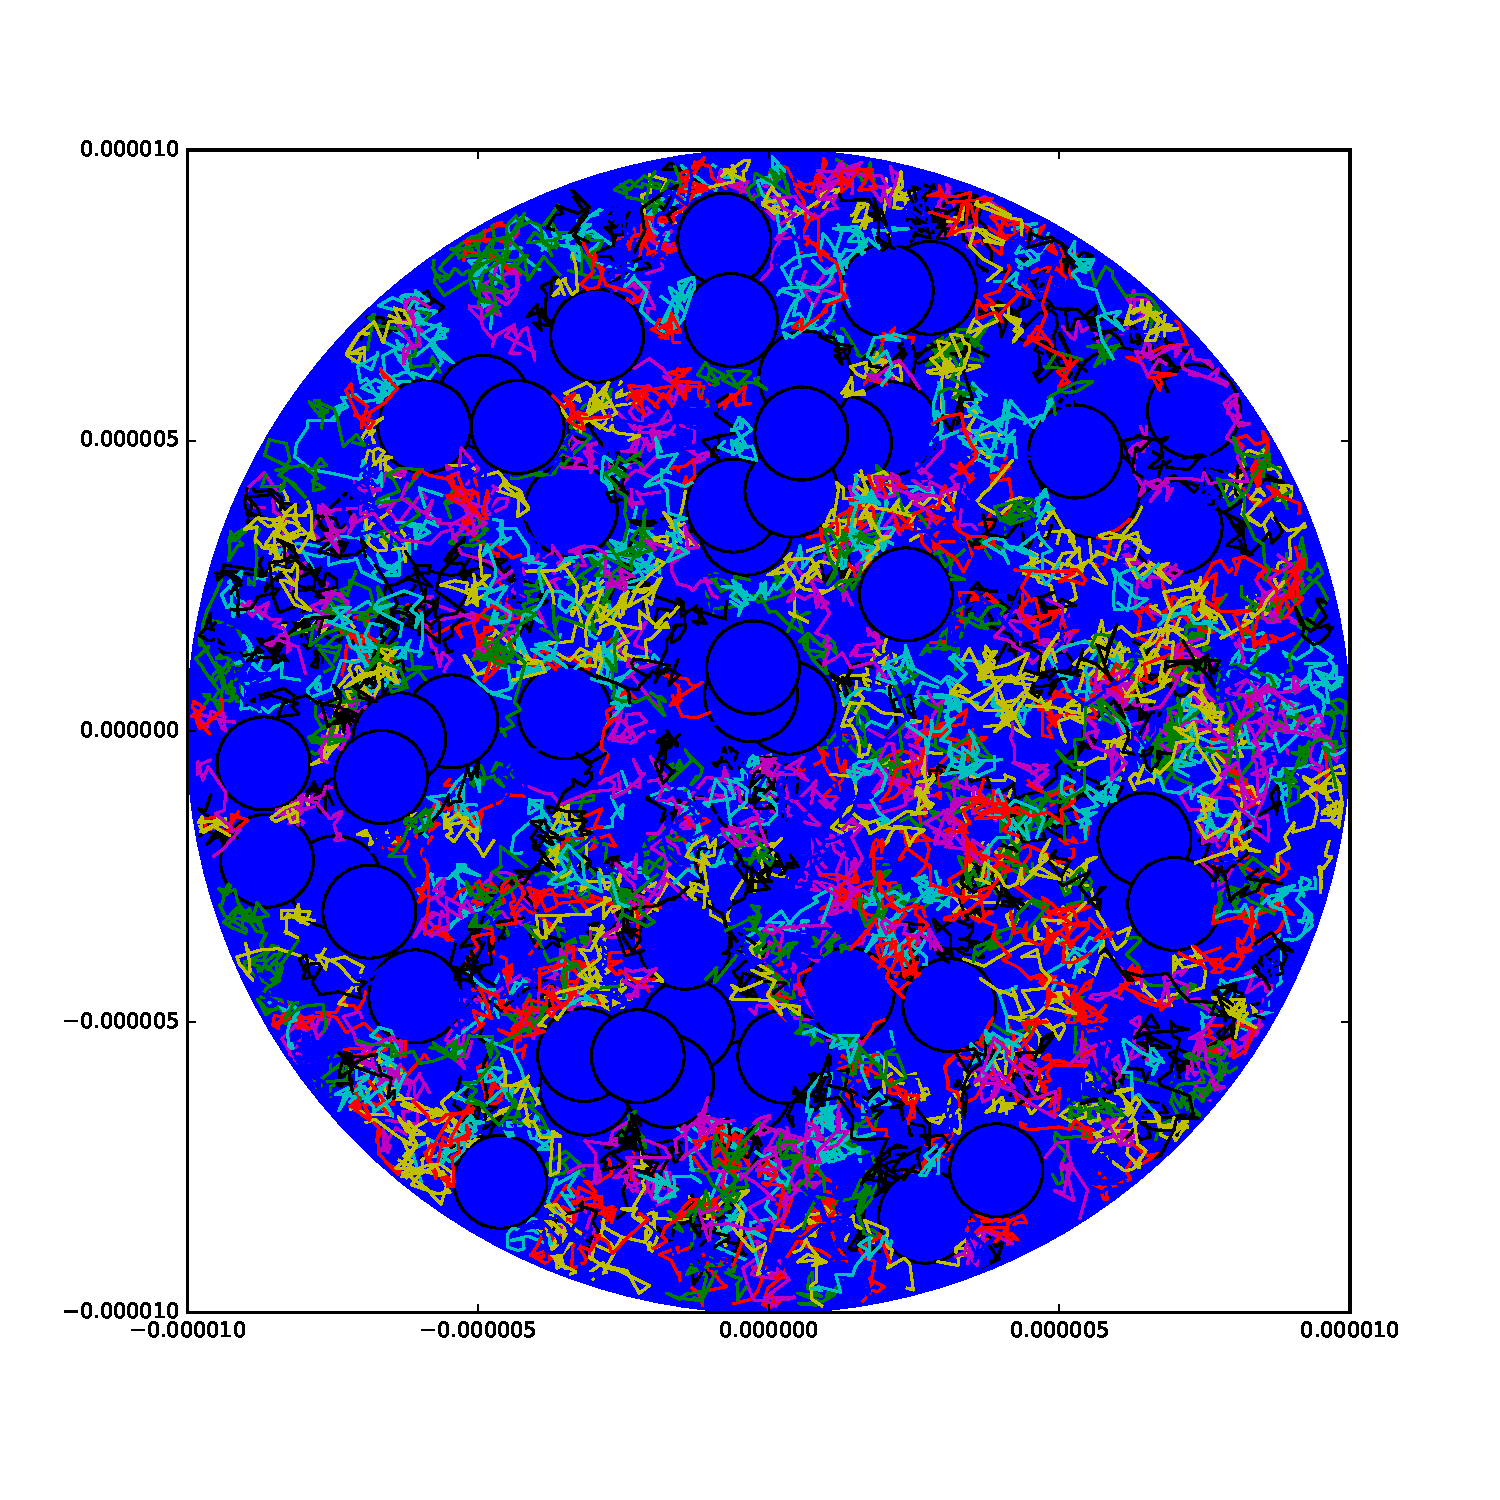
\includegraphics{model.pdf}}
		\label{image2}
	\end{figure}
\end{frame}

\begin{frame}{Метод оптимизации}
	Подбирать наиболее хорошую модель будем при помощи генетического алгоритма.
\end{frame}

\begin{frame}{Планы до конца семестра}
	\begin{enumerate}
	\item Усилить сложность модели клетки
	\item Усилить процесс моделирования 
	\item Получить модель, хорошо описывающую экспериментальные данные 
	\end{enumerate}
\end{frame}

\end{document}

